	\chapter{Anexo}
	\section{Como flashear firmware en el ESP8266}
	
	En este apartado se explicará lo necesario para poder flashear el firmware alojado en mi github \url{https://github.com/Miguelmoral/ESP8266-energy-monitor/tree/master/firmware} en la placa ESP8266.
	
	En primer lugar tendremos que descargar el programa Arduino IDE desde la web oficial \cite{arduinoide}.
	
	Una vez instalada cualquiera de las versiones de Arduino IDE veremos que la placa ESP8266 no se encuentra disponible entre el listado de placas por defecto que nos permite seleccionar el IDE por lo que tendremos que instalar un plugin para utilizar dicha placa. En el menú Archivo/Preferencias veremos un apartado donde podremos escribir llamado Gestor de URLs Adicionales de Tarjetas donde introduciremos esta URL \url{http://arduino.esp8266.com/stable/package_esp8266com_index.json}.
	
	\begin{figure}[H]
		\centering
		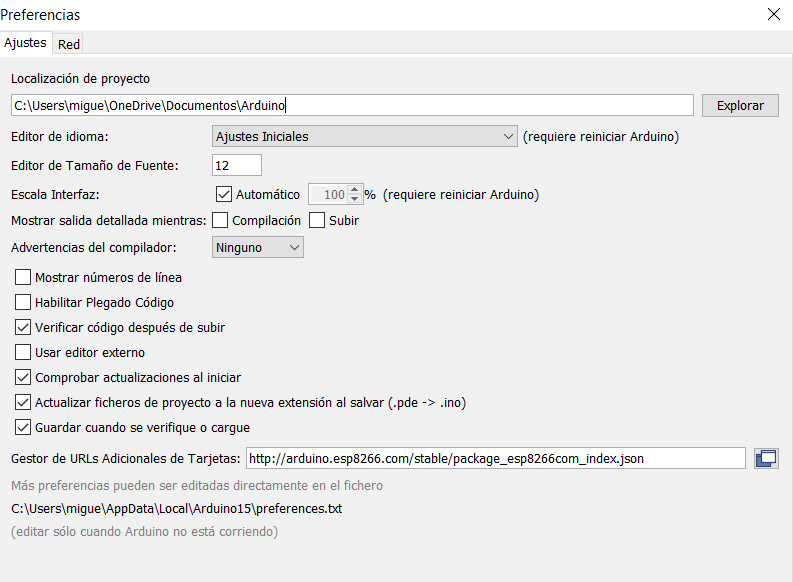
\includegraphics[scale=0.6]{imagenes/preferenciasarduino.png}
		\caption{Archivo/Preferencias}
		\label{fig:preferenciasarduino}
	\end{figure}
	
	Una vez agregada la URL accedemos a Herramientas/Placa/Gestor de tarjetas y buscamos e instalamos esp8266 by ESP8266 community (\ref{fig:instalarESP8266}).
	
	\begin{figure}[H]
		\centering
		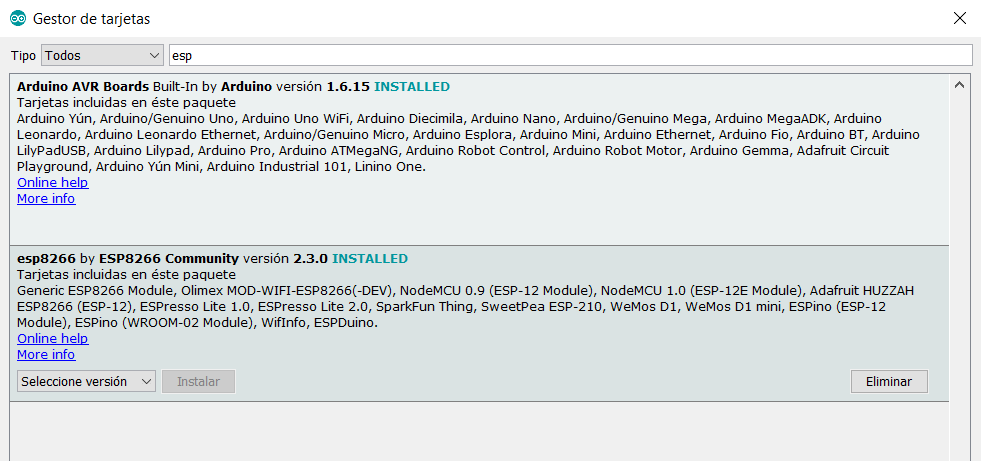
\includegraphics[scale=0.6]{imagenes/instalarESP.png}
		\caption{Herramientas/Placa/Gestor de tarjetas}
		\label{fig:instalarESP8266}
	\end{figure}
	
	En este momento tan solo nos faltará abrir el archivo .ino descargado previamente de github el cuál contiene el firmware actualizando el servidor donde queremos que se manden los datos recogidos por el sensor y las credenciales de nuestra red Wifi para que la placa ESP8266 tenga acceso a la red y pulsar sobre el botón subir para flashear el firmware a la placa.

